\documentclass[tikz]{standalone}
\usepackage{tikz}
\usetikzlibrary{positioning, graphs}
\usetikzlibrary{graphs.standard}
\begin{document}
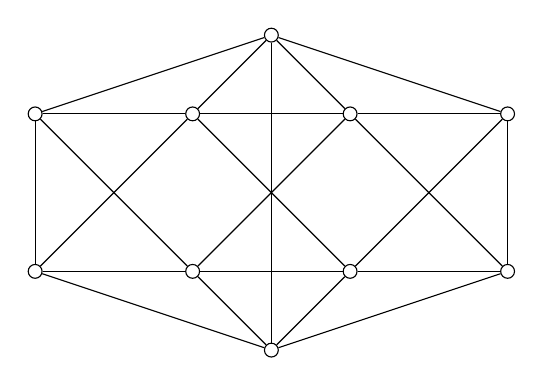
\begin{tikzpicture}
\begin{scope}
		[vertex/.style={draw,circle,inner sep = 0em, minimum size = 0.5em}, node distance = 1em]
		\node[vertex] (a) at (0,0) {};
		\node[vertex] (b) at (2,0) {};
		\node[vertex] (c) at (4,0) {};
		\node[vertex] (d) at (6,0) {};
		\node[vertex] (e) at (0,2) {};
		\node[vertex] (f) at (2,2) {};
		\node[vertex] (g) at (4,2) {};
		\node[vertex] (h) at (6,2) {};
		\node[vertex] (i) at (3,3) {};
		\node[vertex] (j) at (3,-1) {};
		
		\draw[-] (a) to (b);
		\draw[-] (b) to (c);
		\draw[-] (c) to (d);
		\draw[-] (d) to (h);
		\draw[-] (h) to (g);
		\draw[-] (g) to (f);
		\draw[-] (f) to (e);
		\draw[-] (e) to (a);
		\draw[-] (a) to (f);
		\draw[-] (e) to (b);
		\draw[-] (b) to (g);
		\draw[-] (f) to (c);
		\draw[-] (c) to (h);
		\draw[-] (g) to (d);
		\draw[-] (i) to (e);
		\draw[-] (i) to (f);
		\draw[-] (i) to (g);
		\draw[-] (i) to (h);
		\draw[-] (j) to (a);
		\draw[-] (j) to (b);
		\draw[-] (j) to (c);
		\draw[-] (j) to (d);
		\draw[-] (i) to (j);
\end{scope}
\end{tikzpicture}
\end{document}